% acmtr.tex
% revised 1/20/97
% updated 06/01/01
% $Header: acmtr.tex,v 1.5 2/14/96 11:07:57 boyland Exp $

\documentclass[acmtocl]{acmtrans2m}
%&t&{\tt #}&
%&v&\verb|#|&

\acmVolume{2}
\acmNumber{3}
\acmYear{01}
\acmMonth{09}
\usepackage[utf8]{inputenc}
\usepackage{graphicx}
\usepackage{amsmath}
\usepackage{algorithmic}
\usepackage{algorithm}
\usepackage{url}


\newcommand{\BibTeX}{{\rm B\kern-.05em{\sc i\kern-.025em b}\kern-.08em
    T\kern-.1667em\lower.7ex\hbox{E}\kern-.125emX}}
\newcommand{\titulo}{KD-Tree Based Load Balancing for MMOG servers}
\newcommand{\autores}{Carlos Eduardo B. Bezerra, João L. D. Comba and Cláudio F. R. Geyer}
%\markboth{Leslie Lamport et al.}{Preparing Articles for the ACM 
\markboth{\autores}{\titulo}

\title{\titulo}
\author{CARLOS EDUARDO B. BEZERRA\\JOÃO L. D. COMBA\\CLÁUDIO F. R. GEYER\\Universidade Federal do Rio Grande do Sul}
%\author{Carlos Eduardo B. Bezerra\\Digital Equipment Corporation\\
%ANDREW W. APPEL\\Princeton University \and
%JOHN TANG BOYLAND\\University of California, Berkeley}
\begin{abstract}
MMOGs (massively multiplayer online games) are applications that require high bandwidth connections to work properly. This demand for bandwidth is specially critical on the servers that host the game. This happens because the typical number of simultaneous participants in this kind of game varies from a few hundreds to several tens of thousands, and the server is the one responsible for mediating the interaction between every pair of players connected to it. To deal with this problem, decentralized architectures with multiple servers have been proposed, where each server manages a region of the virtual environment of the game. Each player, then, connects only to the server that manages the region where he is playing. However, to distribute the load among the servers, it is necessary to devise an algorithm for partitioning the virtual environment. In order to readjust the load distribution during the game, this algorithm must be dynamic. Some work has already been made in this direction, but with a geometric algorithm, more appropriate than those found in the literature, it should be possible to reduce the distribution granularity without compromising the rebalancing time, or even reducing it. In this work, we propose the use of a kd-tree for dividing the virtual environment of the game into regions, each of which being designated to one of the servers. The split coordinates of the regions are adjusted dynamically according to the distribution of avatars in the virtual environment. We compared our algorithm to some approaches found in the literature and the simulation results show that our algorithm performed better in most aspects we analyzed.
\end{abstract}

\category{D.2.7}{Software Engineering}{Distribution and 
Main\-ten\-ance}%
[documentation]

\category{H.4.0}{Information Systems Applications}{General}

\category{I.7.2}{Text Processing}{Document Preparation}[languages \and
  photocomposition]

\terms{Documentation, Languages}

\keywords{MMOGs, load balancing, distributed server, kd-trees}



\begin{document}


\setcounter{page}{111}

%\begin{bottomstuff}
%Author's address: L. Lamport, System Research Center,
%Digital Equipment Corporation, 130 Lytton Ave., Palo Alto, CA 
%94301.\newline
%Start of a second footnote ...
%\end{bottomstuff}
\maketitle


\section{Introduction}

The main characteristic of MMOGs is the large number of players interacting simultaneously, reaching the number of tens of thousands \cite{schiele2007rpp}. When using a client-server architecture for the players to communicate with one another, the server intermediates the communication between each pair of players.

To allow the interaction of players, each one of them sends his commands to the server, which calculates the resulting game state and sends it to all the players to whom the state change is relevant. We can see that the number of state update messages sent by the server may grow proportionally to the square of the number of players, if all players are interacting with one another. Obviously, depending on the number of players, the cost of maintaining a centralized infrastructure like this is too high, restricting the MMOG market to large companies with enough resources to pay the upkeep of the server.

In order to reduce this cost, several decentralized solutions have been proposed. Some of them use peer-to-peer networks, such as \cite{schiele2007rpp,rieche2007ppb,hampel2006ppa,elrhalibi2005abm,iimura2004zfg,knutsson2004pps}. Others propose the use of a distributed server composed of low-cost nodes connected through the Internet, as in \cite{ng2002msa,chertov:olb,lee2003sdl,assiotis2006dam}. Anyway, in all these approaches, the ``world'', or virtual environment of the game is divided into regions and for every region is assigned a server -- or a group of peers to manage it, when using peer-to-peer networks. Each of these regions must have a content such that the load imposed on the corresponding server is not greater than its capacity.

When an \emph{avatar} (representation of the player in the virtual environment) is located in a region, the player controlling that avatar connects to the server associated to that region. That server, then, is responsible for receiving the input from that player and for sending, in response, the update messages. When a server becomes overloaded due to an excessive number of avatars in its region and, therefore, more players to be updated, the division of the virtual environment must be recalculated in order to alleviate the overloaded server.

Usually, the virtual environment is divided into relatively small cells, which are then grouped into regions and distributed among the servers. However, this approach has a severe limitation in its granularity, since the cells have fixed size and position. Using a more appropriate geometric algorithm, it should be possible to achieve a better player distribution among different servers, making use of traditional techniques that are generally used for computer graphics.

In this work, we propose the utilization of a kd-tree to perform the partitioning of the virtual environment. When a server is overloaded, it triggers the load balancing, readjusting the limits of its region by changing the split coordinates stored in the kd-tree. A prototype has been developed and used in simulations. The results found in these simulations have been compared to previous results from approaches which use the cell division technique.

The text is organized as follows: in section \ref{context}, some related works are described; in section \ref{sec:proposal}, the algorithm proposed here is presented in detail; in the sections \ref{sec:simul} and \ref{sec:result}, we present, respectively, the simulation details and its results and, in section \ref{sec:conc}, the conclusions of this work are presented.


\section{Related Work}
\label{context}

Different authors have tried to address the problem of partitioning the virtual environment in MMOGs for distribution among multiple servers \cite{ahmed2008mol,bezerra2009lbs}. Generally, there is a static division into cells of fixed size and position. The cells are then grouped into regions (Figure \ref{fig:cells}), and each region is delegated to one of the servers. When one of them is overwhelmed, it seeks other servers, which can absorb part of the load. This is done by distributing one or more cells of the overloaded server to other servers.

\begin{figure}[!t]
	\centering
	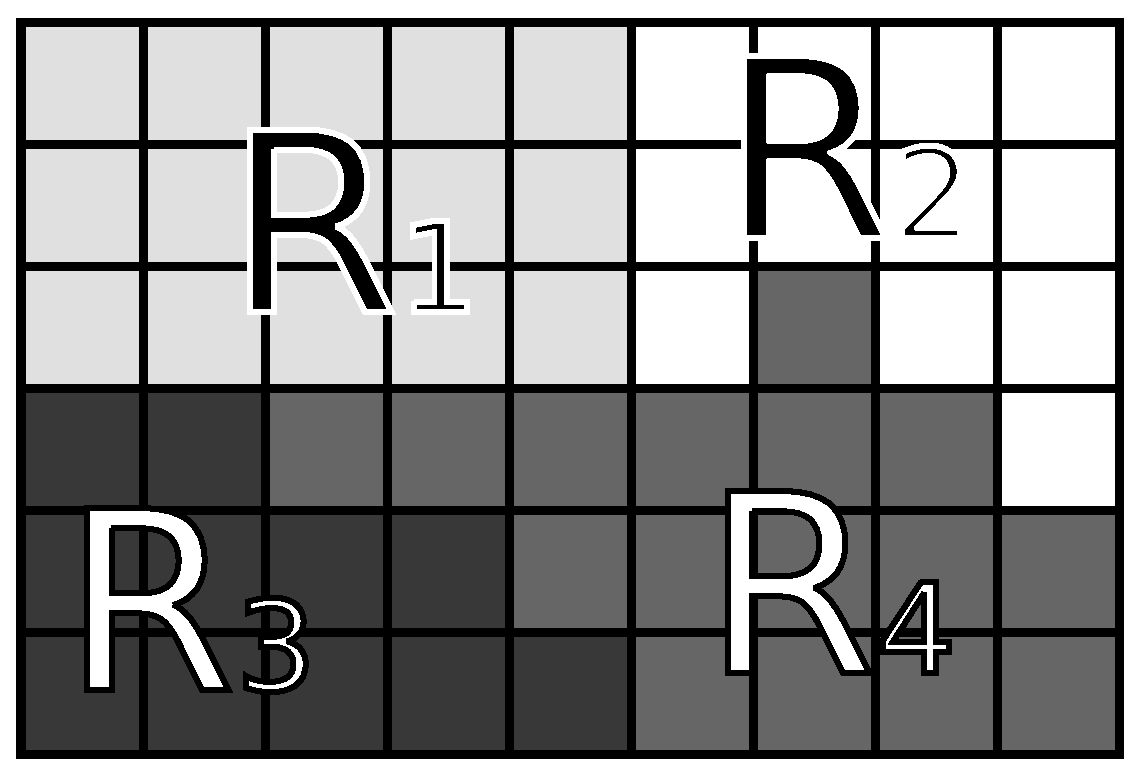
\includegraphics[width=0.85\linewidth]{images/macromicro}
	\caption{Division into cells and grouping into regions}
	\label{fig:cells}
\end{figure}

\cite{ahmed2008mol}, for example, propose a cell-oriented load balancing model. To balance the load, their algorithm finds, first, all clusters of cells that are managed by the overloaded server. The smallest cluster is selected and, from this cluster, it is chosen the cell which has the least interaction with other cells of the same server -- the interaction between two cells A and B is defined by the authors as the number of pairs of avatars interacting with each other, one of them in A and the other one in B. The selected cell is then transferred to the least loaded server, considering ``load'' as the bandwidth used to send state updates to the players whose avatars are positioned in the cells managed by that server. This process is repeated until the server is no longer overloaded or there is no more servers capable of absorbing more load -- in this case, one option could be to reduce the frequency at which state update messages are sent to the players, as suggested by \cite{bezerra2008a3}.

\begin{figure}[!t]
	\centering
	\includegraphics[width=0.5\linewidth]{images/grafo}
	\caption{Graph representation of the virtual environment}
	\label{fig:graph}
\end{figure}

In \cite{bezerra2009lbs}, it is also proposed the division into cells. To perform the division, the environment is represented by a graph (Figure \ref{fig:graph}), where each vertex represents a cell. Every edge in the graph connects two vertices representing neighboring cells. The weight of a vertex is the server's bandwidth occupied to send state updates to the players whose avatars are in the cell represented by that vertex. The interaction between any two cells define the weight of the edge connecting the corresponding vertices. To form the regions, the graph is partitioned using a greedy algorithm: starting from the heaviest vertex, at each step it is added the vertex connected by the heaviest edge to any of the vertices already selected, until the total weight of the partition of the graph -- defined as the sum of the vertices' weights -- reaches a certain threshold related to the total capacity of the server that will receive the region represented by that partition of the graph.

Although this approach works, there is a serious limitation on the distribution granularity it can achieve. If a finer granularity is desired, it is necessary to use very small cells, increasing the number of vertices in the graph that represents the virtual environment and, consequently, the time required to perform the balancing. Besides, the control message containing the list of cells designated to each server also becomes longer. Thus, it may be better to use another approach to perform the partitioning of the virtual environment, possibly using a more suitable data structure, such as the kd-tree \cite{bentley1975mbs}.

This kind of data structure is generally used in computer graphics. However, as in MMOGs there is geometric information -- such as the position of the avatars in the environment --, space partitioning trees can be used. Moreover, we cand find in the literature techniques for keeping the partitions defined by the tree with a similar ``load''. In \cite{luque2005bpc}, for example, it is sought to reduce the time needed to calculate the collisions between pairs of objects moving through space. The authors propose the use of a BSP (binary space partitioning) tree to distribute the objects in the scene (Figure \ref{fig:bsp}). Obviously, if each object of a pair is completely inserted in a different partition, they do not collide and there is no need to perform a more complex test for this pair. Assuming an initial division, it is proposed by the authors a dynamic readjustment of the tree as objects move, balancing their distribution on the leaf-nodes of the tree and, therefore, minimizing the time required to perform the collision detection. Some of the ideas proposed by the authors may be used in the context of load balancing between servers in MMOGs.

\begin{figure}[!t]
	\centering
	\includegraphics[width=0.5\linewidth]{images/bsp}
	\caption{Space partitioning using a BSP tree}
	\label{fig:bsp}
\end{figure}

\section{Proposed approach}
\label{sec:proposal}

The load balancing approach proposed here is based on two criteria: first, the system should be considered heterogeneous (i.e. every server may have a different amount of resources) and, second, the load on each server is \emph{not} proportional to the number of players connected to it, but to the amount of bandwidth required to send state update messages to them.

This choice is due to the fact that every player sends commands to the server at a constant rate, so the number of messages received by the server per unit time grows linearly with the number of players, whereas the number of state update messages sent by the server may be quadratic, in the worst case.

As mentioned in the introduction, to divide the environment of the game into regions, we propose the utilization of a data structure known as kd-tree. The vast majority of MMOGs, such as World of Warcraft \cite{worldofwarcraft}, Ragnarok \cite{ragnarok} and \mbox{Lineage II} \cite{lineage2}, despite having three-dimensional graphics, the simulated world -- cities, forests, swamps and points of interest in general -- in these games is mapped in two dimensions. Therefore, we propose to use a kd-tree with \mbox{k = 2}.

Each node of the tree represents a region of the space and, moreover, in this node it is stored a split coordinate. Each one of the two children of that node represents a subdivision of the region represented by the parent node, and one of them represents the sub-region before the split coordinate and the other one, the sub-region containing points whose coordinates are greater than or equal to the split coordinate. The split axis (in the case of two dimensions, the axes $x$ and $y$) of the coordinate stored alternates for every level of the tree -- if the first level nodes store x-coordinates, the second level nodes store y-coordinates and so on. Every leaf node also represents a region of the space, but it does not store any split coordinate. Instead, it stores a list of the avatars present in that region. Finally, each leaf node is associated to a server of the game. When a server is overloaded, it triggers the load balancing, which uses the kd-tree to readjust the split coordinates that define its region, reducing the amount of content managed by it.

Every node of the tree also stores two other values: capacity and load of the subtree. The load of a non-leaf node is equal to the sum of the load of its children. Similarly, the capacity of a non-leaf node is equal to the sum of the capacity of its children nodes. For the leaf nodes, these values are the same of the server associated to each one of them. The tree root stores, therefore, the total weight of the game and the total capacity of the server system.

In the following sections, it will be described the construction of the tree, the calculation of the load associated with each server and the proposed balancing algorithm.

\subsection{Building the kd-tree}

To make an initial space division, it is constructed a balanced kd-tree. For this, we use the recursive function shown in Algorithm \ref{alg:buildtree} to create the tree.

\begin{algorithm}
\caption{node::build\_tree(id, level, num\_servers)}
\label{alg:buildtree}
\begin{algorithmic}
	\IF{id + $2^{level} \ge num\_servers$ }
		\STATE $left\_child \leftarrow right\_child \leftarrow NIL$;
		\STATE return;
	\ELSE
		\STATE $left\_child \leftarrow$ new\_node();
		\STATE $left\_child.parent \leftarrow$ \textbf{this};
		\STATE $right\_child \leftarrow$ new\_node();
		\STATE $right\_child.parent \leftarrow$ \textbf{this};
		\STATE $left\_child$.build\_tree$(id, level + 1, num\_servers)$;
		\STATE $right\_child$.build\_tree$(id + 2^{level}, level + 1, num\_servers)$;
	\ENDIF
\end{algorithmic}
\end{algorithm}

\begin{figure}[!t]
	\centering
	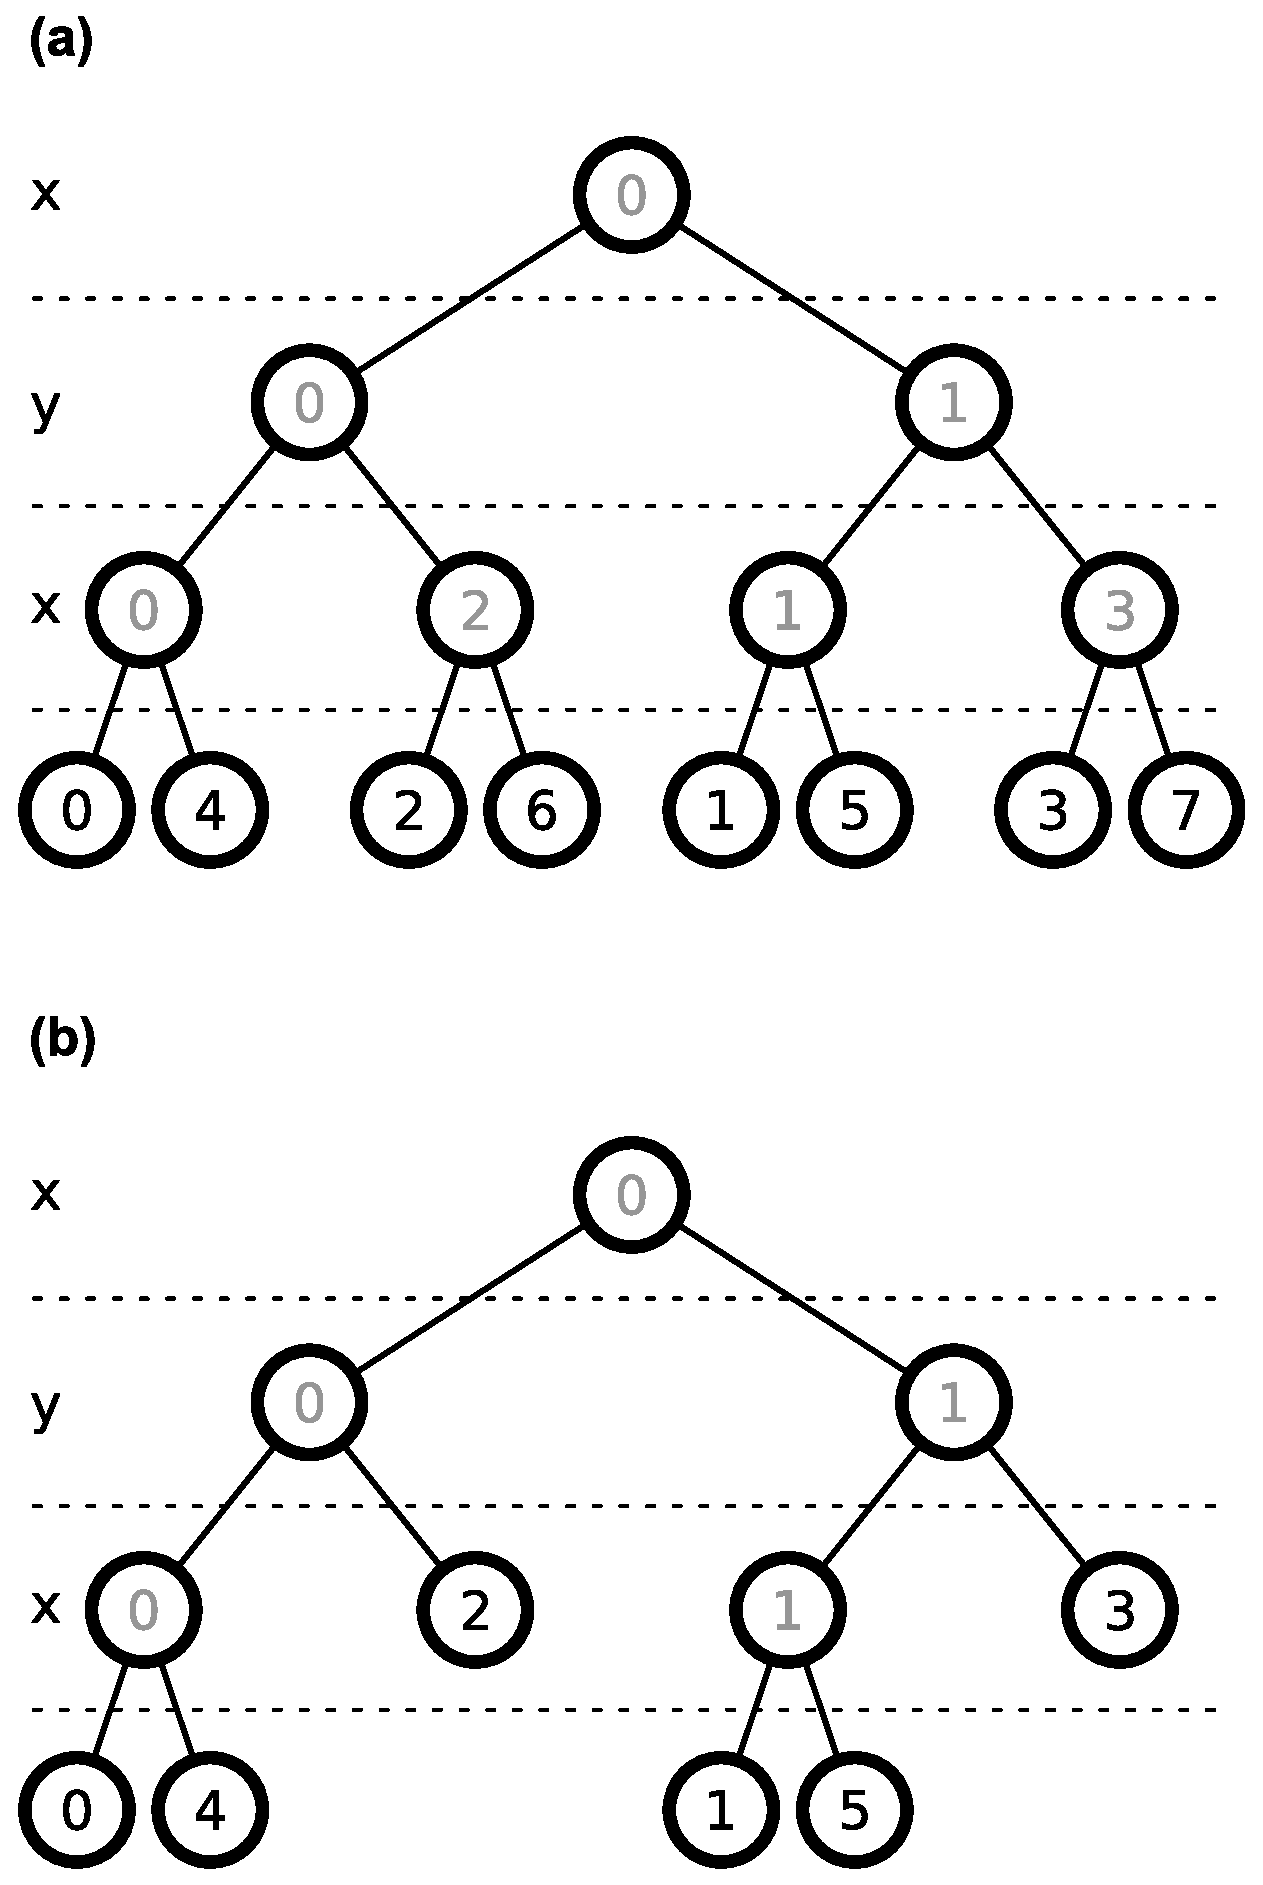
\includegraphics[width=0.75\linewidth]{images/kdtree}
	\caption{Balanced kd-trees built with the described algorithm}
	\label{fig:kdtree}
\end{figure}

In Algorithm \ref{alg:buildtree}, the $id$ value is used to calculate whether each node has children or not and, in the leaf nodes, it determines the server associated to the region represented by each leaf of the tree. The purpose of this is to create a balanced tree, where the number of leaf nodes on each of the two sub-trees of any node differs, in the maximum, by one. In Figure \ref{fig:kdtree} (a), we have a full kd-tree formed with this simple algorithm and, in Figure \ref{fig:kdtree} (b), an incomplete kd-tree with six-leaf nodes. As we can see, every node of the tree in (b) has two sub-trees whose number of leaf nodes differs by one in the worst case.

\subsection{Calculating the load of avatars and tree nodes}

The definition of the split coordinate for every non-leaf node of the tree depends on how the avatars will be distributed among the regions. An initial idea might be to distribute the players among servers, so that the number of players on each server is proportional to the bandwidth of that server. To calculate the split coordinate, it would be enough to simply sort the avatars in an array along the axis used ($x$ or $y$) by the tree node to split the space and, then, calculate the index in the vector, such that the number of elements before this index is proportional to the capacity of the left child and the number of elements from that index to the end of the array is proportional to the capacity of the right child (Figure \ref{fig:vector}). The complexity of this operation is $O(nlogn)$, due to the sorting of avatars.

\begin{figure}
  \centering
  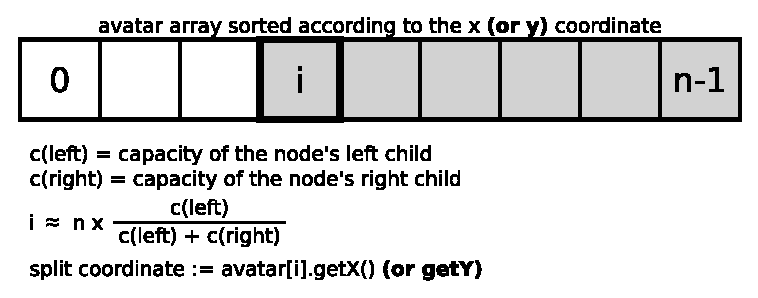
\includegraphics[width=\linewidth]{images/vector}
  \caption{A load splitting considering only the number os avatars}
  \label{fig:vector}
\end{figure}

However, this distribution is not optimal, for the load imposed by the players depends on how they are interacting with one another. For example, if the avatars of two players are distant from each other, there will be probably no interaction between them and, therefore, the server will need only to update every one of them about the outcome of his own actions -- for these, the growth in the number of messages is linear with the number of players. On the other hand, if the avatars are close to each other, each player should be updated not only about the outcome of his own actions but also about the actions of every other player -- in this case, the number of messages may grow quadratically with the number of players \mbox{(Figure \ref{fig:load})}. For this reason, it is not sufficient only to consider the number of players to divide them among the servers.

\begin{figure}
  \centering
  
\includegraphics[width=0.8\linewidth]{images/carga}
  \caption{Relation between avatars and load}
  \label{fig:load}
\end{figure}

A more appropriate way to divide the avatars is by considering the load imposed by each one of them on the server. A brute-force method for calculating the loads would be to get the distance separating each pair of avatars and, based on their interaction, calculate the number of messages that each player should receive by unit of time. This approach has complexity $O(n^2)$. However, if the avatars are sorted according to their coordinates on the axis used to divide the space in the kd-tree, this calculation may be performed in less time.

For this, two nested loops are used to sweep the avatars array, where each of the avatars contains a $load$ variable initialized with zero. As the vector is sorted, the inner loop may start from an index before which it is known that no avatar $a_j$ has relevance to that being referenced in the outer loop, $a_i$. It is used a variable $begin$, with initial value of zero: if the coordinate of $a_j$ is smaller than that of $a_i$, with a difference greater than the maximum view range of the avatars, the variable $begin$ is incremented. For every $a_j$ which is at a distance smaller than the maximum view range, the $load$ of $a_i$ is increased according to the relevance of $a_j$ to $a_i$. When the inner loop reaches an avatar $a_j$, such that its coordinate is greater than that of $a_i$, with a difference greater than the view range, the outer loop moves immediately to the next step, incrementing $a_i$ and setting the value of $a_j$ to that stored in $begin$ (Figure \ref{fig:sweep}).

Let $width$ be the length of the virtual environment along the axis used for the splitting; let also $radius$ be the maximum view range of the avatars, and $n$, the number of avatars. The number of relevance calculations, assuming that the avatars are uniformly distributed in the virtual environment is \mbox{$O(m \times n)$}, where $m$ is the number of avatars compared in the internal loop, i.e. \mbox{$m = \frac{2 \times radius \times n}{width}$}. The complexity of sorting the avatars along one of the axes is $O(nlogn)$. Although it is still quadratic, the execution time is reduced significantly, depending on the size of the virtual environment and on the view range of the avatars. The algorithm could go further and sort each set of avatars $a_j$ which are close (in one of the axes) to $a_i$ according to the other axis and, again, perform a sweep eliminating those which are too far away, in both dimensions. The number of relevance calculations would be \mbox{$O(p \times n)$}, where $p$ is the number of avatars close to $a_i$, considering the two axes of coordinates, i.e. \mbox{$p = \frac{(2 \times radius)^2 \times n}{width \times height}$}. In this case, $height$ is the extension of the environment in the second axis taken as reference. Although there is a considerable reduction of the number of relevance calculations, it does not pay the time spent in sorting the sub-array of the avatars selected for each $a_i$. Adding up all the time spent on sort operations, it would be obtained a complexity of: \mbox{$O(nlogn + n \times mlogm)$}.

\begin{figure}
  \centering
  \includegraphics[width=0.8\linewidth]{images/sweep}
  \caption{Sweep of the sorted array of avatars}
   \label{fig:sweep}
\end{figure}

After calculating the load generated by each avatar, this value is used to define the load on each leaf node and, recursively, on the other nodes of the kd-tree. To each leaf node a server and a region of the virtual environment are assigned. The load of the leaf node is equal to the server's bandwidth used to send state updates to the players controlling the avatars located in its associated region. This way, the load of each leaf node is equal to the sum of the weights of the avatars located in the region represented by it.

\subsection{Dynamic load balancing}

Once the tree is built, each server is associated to a leaf node -- which determines a region. All the state update messages to be sent to players whose avatars are located in a region must be sent by the corresponding server. When a server is overloaded, it may transfer part of the load assigned to it to some other server. To do this, the overloaded server collects some data from other servers and, using the kd-tree, it adjusts the split coordinates of the regions.

Every server maintains an array of the avatars located in the region managed by it, sorted according to the $x$ coordinate. Also, each element of the array stores a pointer to another element, forming a chained list that is ordered according to the $y$ coordinated of the avatars (Figure \ref{fig:vectorxlisty}). By maintaining a local sorted avatar list on each server, the time required for balancing the load is somewhat reduced, for there will be no need for the server performing the rebalance to sort again the avatar lists sent by other servers. It will need only to merge all the avatars lists received from the other servers in an unique list, used to define the limits of the regions, what is done by changing the split coordinates which define the space partitions.

\begin{figure}
  \centering
  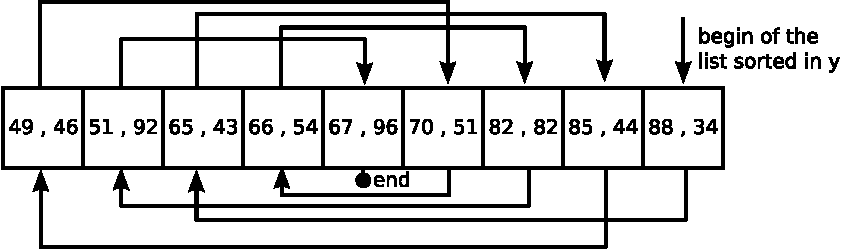
\includegraphics[width=0.9\linewidth]{images/vectorxlisty}
  \caption{Avatar array sorted by x, containing a list sort by y}
   \label{fig:vectorxlisty}
\end{figure}

When the overloaded server initiates the rebalance, it runs an algorithm that traverses the kd-tree, beginning from the leaf node that defines its region and going one level up at each step until it finds an ancestor node with a capacity greater then or equal to the load. While this node is not found, the algorithm continues recursively up the tree until it reaches the root. For each node visited, a request for the information about all the avatars and the values of load and capacity is sent to the servers represented by the leaf nodes of the sub-tree to the left of that node (Figure \ref{fig:ancestors}). With these data, and its own list of avatars and values of load and capacity, the overloaded server can calculate the load and capacity of its ancestral node visited in the kd-tree, which are not known beforehand -- these values are sent on-demand to save up some bandwidth of the servers and to keep the system scalable.

\begin{figure}
  \centering
  \includegraphics[width=0.9\linewidth]{images/ancestors}
  \caption{Search for an ancestor node with enough resources}
   \label{fig:ancestors}
\end{figure}

Reaching an ancestral node with capacity greater than or equal to the load -- or the root of the tree, if no such node is found -- the server that initiated the balance adjusts the split coordinates of the kd-tree nodes. For each node, it sets the split coordinate in a way such that the avatars are distributed according to the capacity of the node's children. For this, it is calculated the load fraction that should be assigned to each child node. The avatar list is then swept, stopping at the index $i$ such that the total load of the avatars before $i$ is approximately equal to the value defined as the load to be designated to the left child of the node whose split coordinate is being calculated (Figure \ref{fig:balancenode}). The children nodes have also, in turn, their split coordinates readjusted recursively, so that they are checked for validity -- the split coordinate stored in a node must belong to the region defined by its ancestors in the kd-tree -- and readjusted to follow the balance criteria defined.

\begin{figure}
  \centering
  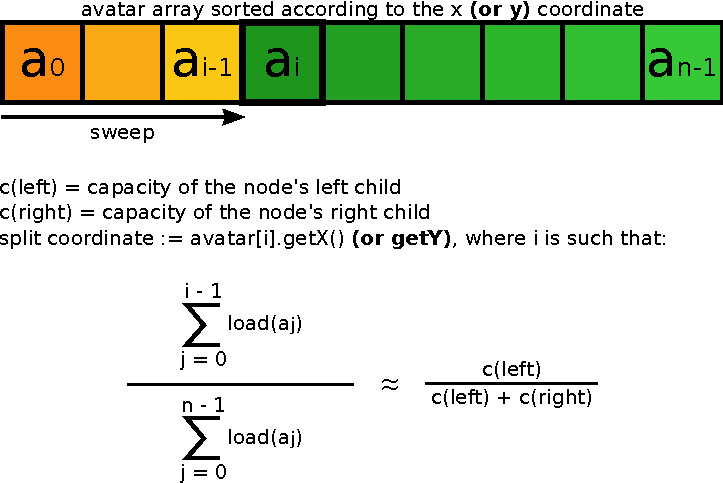
\includegraphics[width=0.9\linewidth]{images/balancenode}
  \caption{Division of an avatar list between two brother nodes}
   \label{fig:balancenode}
\end{figure}

As the avatar lists received from the other servers are already sorted along both axes, it is enough to merge these structures with the avatar list of the server which initiated the rebalance. Assuming that each server already calculated the weight of each avatar managed by it, the rebalance time is  $O(nlogS)$, where $n$ is the number of avatars in the game and $S$ is the number of servers. The communication cost is $O(n)$, caused by the sending of data related to te $n$ avatars. The merging of all avatar lists has $O(n)$ complexity, for the avatars were already sorted by the servers. At each level of the kd-tree, $O(n)$ avatars are swept in the worst case, in order to find the $i$ index whose avatar's coordinate will be used to split the regions defined by each node of the tree (Figure \ref{fig:balancenode}). As this is a balanced tree with $S$ leaf nodes, it has a height of $\lceil logS \rceil$.

\section{Simulations}
\label{sec:simul}

To evaluate the proposed dynamic load balancing algorithm, a virtual environment across which many avatars moved was simulated. Starting from a random point in the environment, each avatar moved according to the random waypoint model \cite{bettstetter2004spr}. To force a load imbalance and stress the algorithms tested, we defined some \emph{hotspots} -- points of interest to which the avatars moved with a higher probability than to other parts of the map. This way, a higher concentration of avatars was formed in some areas. Although the movement model used is not very realistic in terms of the way the players move their avatars in real games, it was only used to verify the load balance algorithms simulated. For each algorithm tested, we simulated two situations: one with the presence of hotspots and one without hotspots.

The proposed approach was compared to the ones presented in section \ref{context}, from other authors. However, it is important to observe that the model employed by \cite{ahmed2008mol} considers hexagonal cells, while in our simulations we used rectangular cells. Furthermore, the authors considered that there is a transmission rate threshold, which is the same for all servers in the system. As we assume a heterogenous system, their algorithm was simulated considering that each server has its own transmission rate threshold, depending on the upload bandwidth available in each one of them. However, we kept what we consider the core idea of the authors' approach, which is the selection of the smallest cell cluster managed by the overload server, then choosing that cell with the lowest interaction with other cells of the same server, and finally the transferring of this cell to the least loaded server. Besides Ahmed's algorithm, we also simulated some of the ones proposed in \cite{bezerra2009lbs} -- Progrega and BFBCT.

The simulated virtual environment consisted of a two-dimensional space, with 750 moving avatars, whose players were divided among eight servers ($S_1, S_2, ..., S_8$), each of which related to one of the regions determined by the balancing algorithm. For the cell-oriented approaches simulated, the space was divided into a \mbox{15 $\times$ 15} cell grid, or 225 cells. The capacity of each server $S_i$ was equal to $i \times 20000$, forming a heterogeneous system. This heterogeneity allowed us to evaluate the load balancing algorithms simulated according to the criterion of proportionality of the load distribution on the servers.

In addition to evaluate the algorithms according to the proportionality of the load distribution, it was also considered the number of player migrations between servers. Each migration involves a player connecting to the new server and disconnecting from the old one. This kind of situation may occur in two cases: the avatar moved, changing the region in which it is located and, consequently, changing the server to which its player is connected; or the avatar was not moving and still its player had to migrate to a new server. In the latter case, obviously the player's transfer was due to a rebalancing. An ideal balancing algorithm performs the load redistribution requiring the minimum possible number of player transfers between servers, while keeping the load on each server proportional to its capacity.

Finally, the inter-server communication overhead will also be evaluated. It occurs when two players are interacting, but each one of them is connected to a different server. Although the algorithm proposed in this work does not address this problem directly, it would be interesting to evaluate how the load distribution performed by it influences the communication between the servers.

\section{Results}
\label{sec:result}

\begin{figure}[!t]
	\centering
	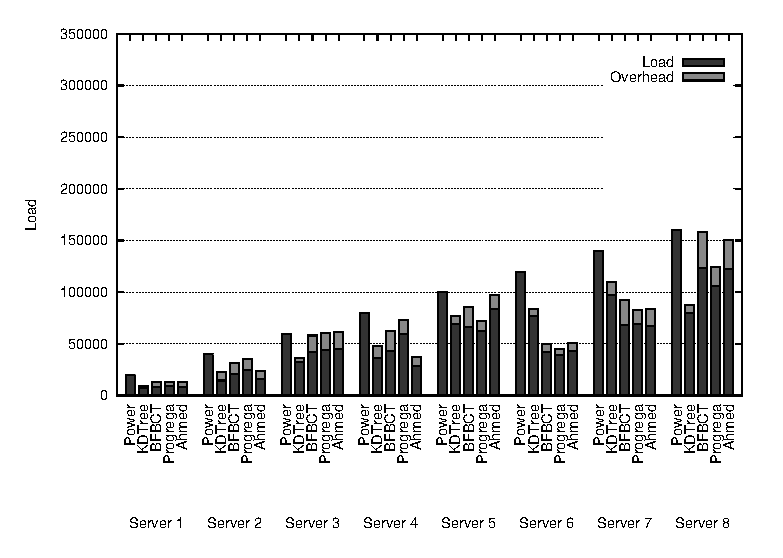
\includegraphics[width=\linewidth]{images/distribution_uniform}
	\caption{Average load on each server (by algorithm, without hotspots)}
	\label{fig:distribution:uniform}
\end{figure}

\begin{figure}[!t]
	\centering
	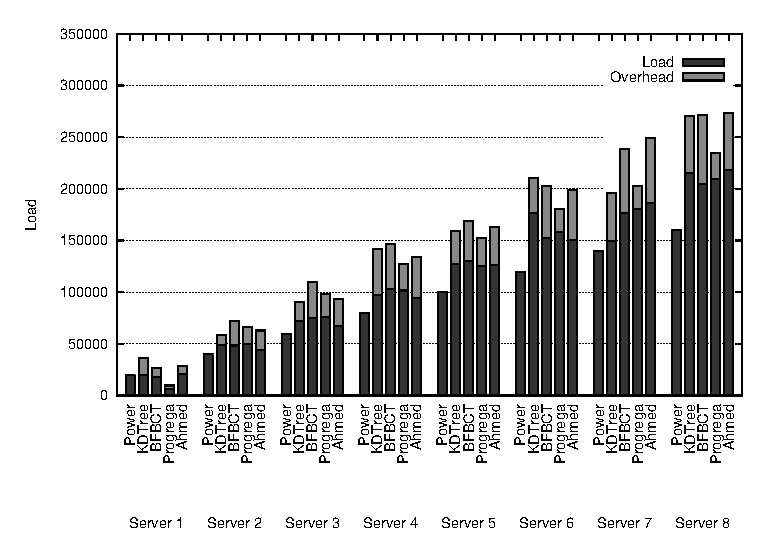
\includegraphics[width=\linewidth]{images/distribution_hotspots}
	\caption{Average load on each server (by algorithm, with hotspots)}
	\label{fig:distribution:hotspots}
\end{figure}

Figures \ref{fig:distribution:uniform} and \ref{fig:distribution:hotspots} present the average load (plus the inter-server communication overhead) on each server, for each algorithm tested. The first figure shows the values in a situation without hotspots and, therefore, a smaller total load. The second, in turn, presents the load distribution when the server system is overloaded. We can see, in Figure \ref{fig:distribution:uniform}, that all algorithms have met the objective of keeping the load on each server less than or equal to its capacity, when the system has sufficient resources to do so. In Figure \ref{fig:distribution:hotspots}, it is demonstrated that all the algorithms managed to dilute -- in a more or less proportional manner -- the load excess on the servers. It is important to observe, however, that the load shown in Figure \ref{fig:distribution:hotspots} is only theoretical. Each server will perform some kind of ``graceful degradation'' in order to keep the load under its capacity. For example, the update frequency might be reduced and access to the game could be denied for new players attempting to join, which is a common practice in most MMOGs.

\begin{figure}[!t]
	\centering
	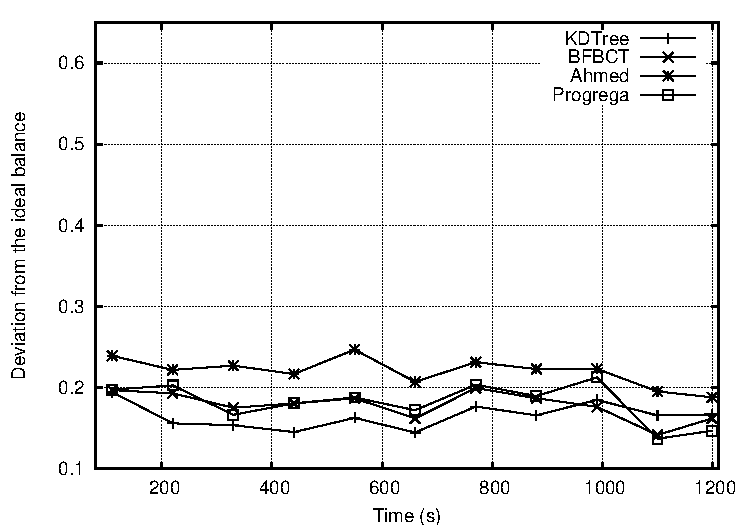
\includegraphics[width=\linewidth]{images/usagedeviation_uniform}
	\caption{Average deviation of the ideal balance of the servers (without hotspots)}
	\label{fig:usagedeviation:uniform}
\end{figure}

\begin{figure}[!t]
	\centering
	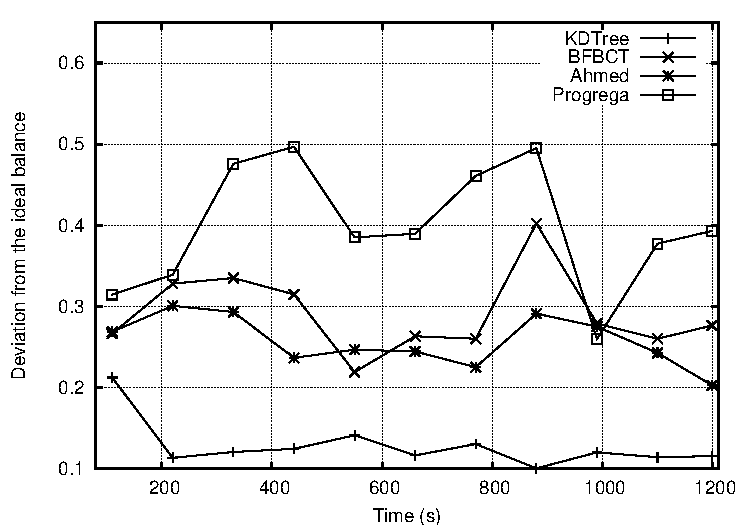
\includegraphics[width=\linewidth]{images/usagedeviation_hotspots}
	\caption{Average deviation of the ideal balance of the servers (with hotspots)}
	\label{fig:usagedeviation:hotspots}
\end{figure}

In figures \ref{fig:usagedeviation:uniform} and \ref{fig:usagedeviation:hotspots}, it is shown how much the balance generated by each algorithm deviates from an ideal balance -- that is, how much, on the average, the load on the servers deviate from a value exactly proportional to the capacity of each one of them -- over time. It is possible to observe that, in both situations -- with and without hotspots -- the algorithm that uses the kd-tree has the least deviation. This is the due to the fine granularity of its distribution, which, unlike the other approaches tested, is not limited by the size of a cell. In the situation with hotspots, the algorithm that uses the kd-tree is particularly effective, because rebalance is needed. In a situation where the system has more resources than necessary, the proportionality of the distribution is not as important: it is enough that each server manages a load smaller than its capacity.

\begin{figure}[!t]
	\centering
	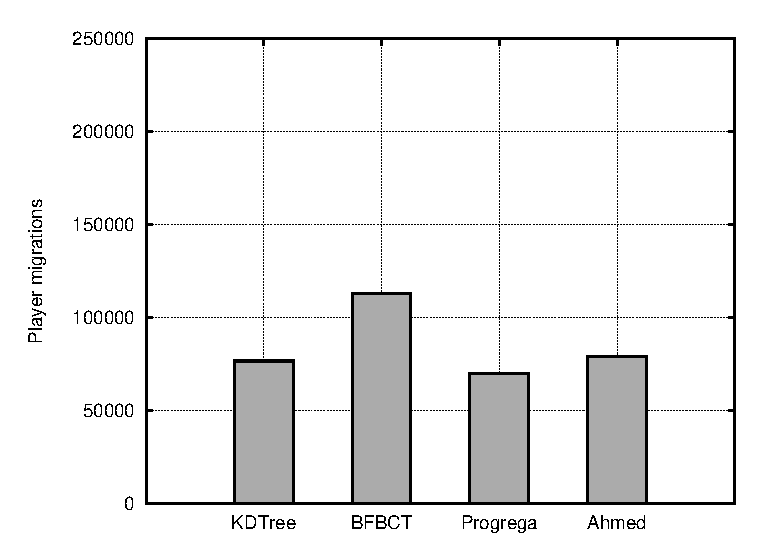
\includegraphics[width=\linewidth]{images/migrations_uniform}
	\caption{Player migrations between servers (without hotspots)}
	\label{fig:migrations:uniform}
\end{figure}

\begin{figure}[!t]
	\centering
	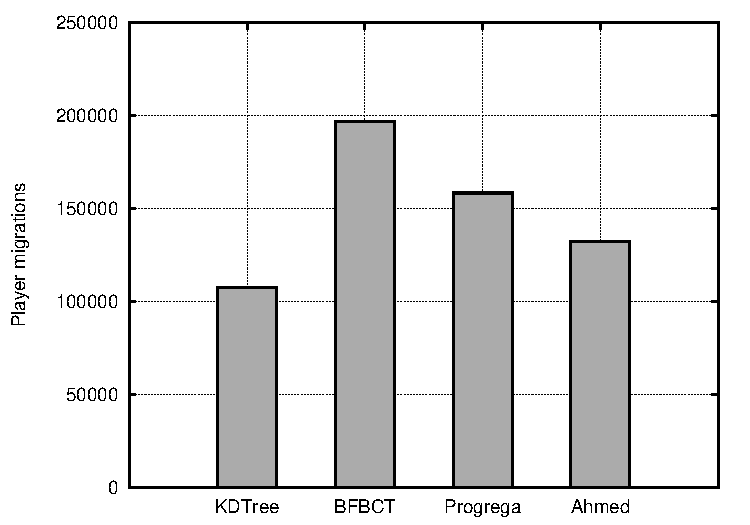
\includegraphics[width=\linewidth]{images/migrations_hotspots}
	\caption{Player migrations between servers (with hotspots)}
	\label{fig:migrations:hotspots}
\end{figure}

Regarding player migrations between servers, all the algorithms -- except BFBCT -- had a similar number of user migrations in the absence of hotspots (Figure \ref{fig:migrations:uniform}). This happens because the load of the game is less than the total capacity of the server system, which required less rebalancing and, thus, caused less migrations of players between servers. Figure \ref{fig:migrations:hotspots}, however, demonstrates that the algorithm that uses the kd-tree had a significantly lower number of user migrations than the other approaches. This is due, in the first place, to the fact that the regions defined by the leaf nodes of the kd-tree are necessarily contiguous, and each server was linked to only one leaf node. An avatar moving across the environment divided into very fragmented regions constantly crosses the borders between these regions and causes, therefore, its player to migrate from server to server repeatedly. Another reason for this result is that each rebalancing executed with the kd-tree gets much closer to an ideal distribution than the cell-based algorithms -- again, thanks to the finer granularity of the kd-tree based distribution --, requiring less future rebalancing and, thus, causing less player migrations.

\begin{figure}[!t]
	\centering
	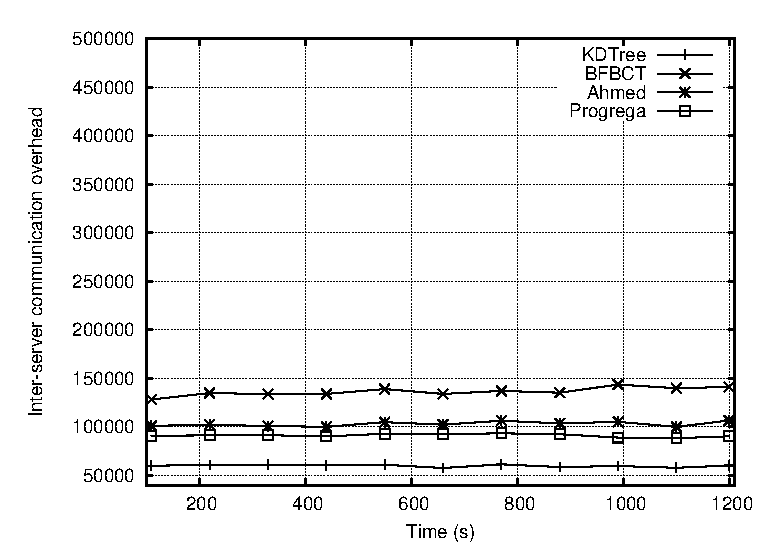
\includegraphics[width=\linewidth]{images/overhead_uniform}
	\caption{Inter-server communication for each algorithm over time (without hotspots)}
	\label{fig:overhead:uniform}
\end{figure}

\begin{figure}[!t]
	\centering
	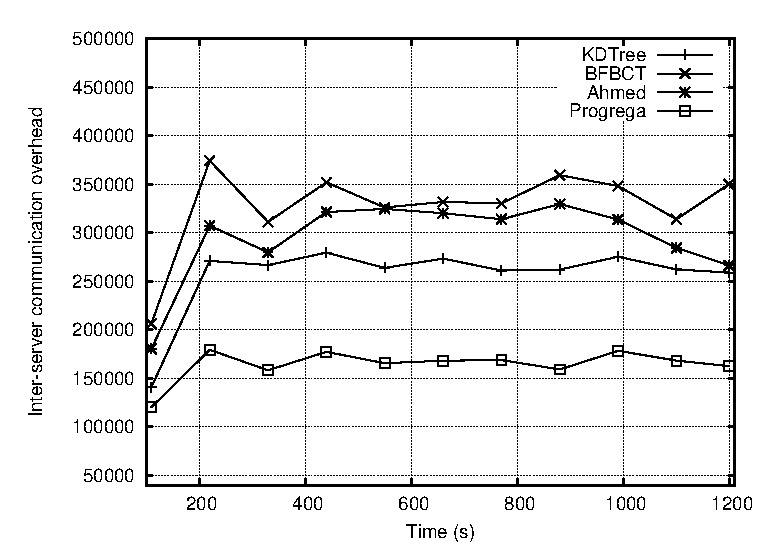
\includegraphics[width=\linewidth]{images/overhead_hotspots}
	\caption{Inter-server communication for each algorithm over time (with hotspots)}
	\label{fig:overhead:hotspots}
\end{figure}

Finally, it is shown the amount of communication between servers for each simulated algorithm, over time. In Figure \ref{fig:overhead:uniform}, all algorithms have similar results, and the one which uses the kd-tree is slightly better than the others. This is also explained by the fact that the regions are contiguous, minimizing the number of boundaries between them and, consequently, reducing the probability of occurring interactions between pairs of avatars, each one in a different region. In Figure \ref{fig:overhead:hotspots}, it is possible to see that the inter-server communication caused by Progrega was considerably lower than all the others in a situation of system overload. The reason for this is that its main goal -- besides balancing the load -- is precisely to reduce the communication between servers. However, even not considering the additional cost, the algorithm that uses the kd-tree got second place in this criterion.

\section{Conclusions}
\label{sec:conc}

In this work, we proposed the use of a kd-tree to partition the virtual environment of MMOGs and perform the load balancing of servers by recursively adjusting the split coordinates stored in its nodes. One of the conclusions reached was that the use of kd-trees to make this partitioning allows a fine granularity of the load distribution, while the readjustment of the regions becomes simpler -- by recursively traversing the tree -- than the common approaches, based on cells and/or graph partitioning.

The finer granularity allows for a better balancing, so that the load assigned to each server is close to the ideal value that should be assigned to it. This better balance also helped to reduce the number of migrations, by performing less rebalancing operations. The fact that the regions defined by the kd-tree are necessarily contiguous was one of the factors that contributed to the results of the proposed algorithm, which was better than the other algorithms simulated in most of the criteria considered.

In conclusion, it was possible to use methods that can reduce the complexity of each rebalancing operation. This is due, first, to the reduction of the number of operations for calculating the relevance between pairs of avatars by sweeping a sorted avatar list and, secondly, to keeping at each server an avatar list already sorted in both dimensions, saving the time that would be spent on sorting the avatars when they were received by the server executing the rebalance.




\section{The Title Page}\label{sec:pag}

\subsection{The Title, Author(s), and Abstract}

Following order is mandatory to generate a correct title
page:\footnote{Section~\ref{sec:pag} has been rewritten by Marco
  Aiello (email: aiellom@acm.org) to explain the new structure of the
  class file as of 2001/06/01. The major novelty is the introduction
  of options for the different transactions and the the automatic
  generation of footers and permission statements.}

% changed w.r.t. original file by K.R.Apt and M.Aiello
\begin{quote}
\begin{verbatim}
\documentclass{acmtrans2m}
            %\acmVolume{V}
            %\acmNumber{N}
            %\acmYear{YY}
            %\acmMonth{Month}
            \markboth{}{}
            \title{}
            \author{}
            \begin{abstract} 
            ...  
            \end{abstract}
            \category{}{}{}
            \terms{} 
            \keywords{}
            \begin{document}
            \begin{bottomstuff} 
            ... 
            \end{bottomstuff}
            \maketitle
\end{verbatim}
\end{quote}
The \verb|\documentclass[journalName]{acmtrans2m}| takes as option the
specific transaction one is preparing. The transactions currently
supported are:

\medskip
\begin{tabular}{l l l}
        option name & journal\\
\hline
        \verb|acmjacm| & Journal of the ACM\\
        \verb|acmtocl| & Transactions on Computational Logic\\
        \verb|acmtodaes| & Transactions on Design Automation of Electronic Systems\\
        \verb|acmtods| & Transactions on Database Systems\\
        \verb|acmtogs| & Transactions on Graphics\\
        \verb|acmtoms| & Transactions on Mathematical Software\\
        \verb|acmtoplas| & Transactions on Programming Languages and Systems\\
\end{tabular}

\medskip\noindent For example, to prepare a manuscript for the
Transactions on Compuational Logic the file should begin with
\begin{quote}
\begin{verbatim}
\documentclass[acmtocl]{acmtrans2m}
\end{verbatim}
\end{quote}


\medskip\noindent
%The additional option \verb|acmnow| generates the current month and
%year in the footers and permission information of the paper.  (This is
%a feature that authors may very well ignore in preparing their
%manuscripts.)
%\begin{quote}
%\begin{verbatim}
%\documentclass[journalName,acmnow]{acmtrans2m}
%\end{verbatim}
%\end{quote}
The four commands
\begin{quote}
\begin{verbatim}
            %\acmVolume{V}
            %\acmNumber{N}
            %\acmYear{YY}
            %\acmMonth{Month}
\end{verbatim}
\end{quote}
are needed to generate footer and copyright information. The commands
store the following information: volume number, issue number, last two
digits of the year of publication, and month name in English,
respectively. The appropriate values will be communicated by the
Editor-in-Chief upon acceptance of the final version of the paper.




\subsubsection{Title and Author}
The \LaTeX\ \verb|\title| and \verb|\author| declarations and the
\verb|\maketitle| command are employed as usual.  However, the user
must format the author a little differently to match the ACM standard.
The following example \cite{6:1:1} illustrates most features:
\begin{quote}
\begin{verbatim}
\author{JAMES E. ARCHER, JR.\\ Rational Machines
        \and RICHARD CONWAY and FRED B. SCHNEIDER \\ 
             Cornell University}
\end{verbatim}
\end{quote}
Note that authors' names are in uppercase letters, authors are
separated from their affiliation by a \verb|\\| command, multiple
authors with the same affiliation are separated by ``and'' (or commas
and ``and'' if there are more than two), and authors with different
affiliations are separated by an \verb|\and| command.  The following
example \cite{6:3:380} shows what to do if there are more than
two affiliations:
\begin{quote}
\begin{verbatim}
\author{E. KORACH \\ IBM Israel \\
        D. ROTEM \\ University of Waterloo
        \and N. SANTORO \\ Carleton University}
\end{verbatim}
\end{quote}
In both the title and the author, you may have to insert \verb|\\|
commands if lines need to be broken. 

\subsubsection{Abstract}
The abstract is typed as usual with the {\tt abstract} environment.
However, this environment must come before the \verb|\maketitle|
command.


\subsection{Content Indicators and Keywords}

The content indicators and keywords are entered with \LaTeX\ 
declarations.  The CR categories are indicated with \verb|\category|
declarations.  The first CR category of this article, appearing
right below the abstract, was entered with the following command:
\begin{quote}
\begin{verbatim}
\category{D.2.7}{Software Engineering}{Distribution and 
  Maintenance}[Documentation]
\end{verbatim}
\end{quote}
Note that the last argument (which contains the subject descriptors)
is optional, since some categories have none.  Multiple subject 
descriptors
are separated by \verb|\and| commands, as in the last category of
this article:
\begin{quote}
\begin{verbatim}
\category{I.7.2}{Text Processing}{Document Preparation}
         [Languages \and Photocomposition]
\end{verbatim}
\end{quote}
Use a separate \verb|\category| declaration for each CR category;
they will be listed in the order that the commands appear.  The
\verb|\category| commands must precede the \verb|\maketitle|
command.

The General Terms are declared with a (single) \verb|\terms|
command as in the one for this article:
\begin{quote}
\begin{verbatim}
\terms{Documentation, Languages}
\end{verbatim}
\end{quote}
The \verb|\terms| declaration must come before the \verb|\maketitle|
command.  The terms {\it must} be chosen from the following list:
\begin{quote}
Algorithms; 
Design; 
Documentation; 
Economics; 
Experimentation; 
Human factors; 
Languages; 
Legal aspects; 
Management; 
Measurement; 
Performance; 
Reliability; 
Security; 
Standardization; 
Theory; 
Verification; 
\end{quote}
The general terms are
orthogonal to the Categories, at least theoretically, and so
may be applied to any elements of the classification tree.

Think of them as `perspectives' from which any topic may
be approached. Thus you could use {\em Theory} or {\em Performance} 
for an
article about {\em C.2.1 Distributed Networks}. However, 
some of these general terms actually slide over into
content areas. Thus {\em Legal aspects} is a general term
applicable to any category, but also an entire node in the tree,
{\em K.5}, devoted to {\em Legal aspects of computing,} with many 
sub-topics.

So, though perhaps not perfect, the General Terms are most useful
in online searches when used in combination with categories.

The ``Additional Keywords and Phrases'' item on the title page
is provided by the \verb|\keywords| declaration, {\bf listed 
alphabetically\/}.
For this article,  
they were produced by the following command:
\begin{quote}
\begin{verbatim}
\keywords{Document preparation, publications, typesetting}
\end{verbatim}
\end{quote}
There is no prescribed list of ``additional keywords;'' use any that
you want.

\subsection{The Bottom of the Title Page}\label{sec:permission}

The bottom of the article's title page contains acknowledgment of
support, the author(s) address(es), a ``permission to copy'' 
statement,
and a line containing a copyright symbol (\copyright) and a mysterious
number.  This is all entered with a {\tt bottomstuff} environment;
there must be no blank line after the \verb|\begin{bottomstuff}|
command.  

\subsection{The Page Headers}

\verb|\markboth{}{}| generates the left- and right-page headers. The 
first 
argument is the author's name(s):

\begin{itemize}
\item If there is one author, then use author's full name (ex. Leslie 
Lamport);
\item If there are two authors, then abbreviate each author's first 
name
           (L.~Lamport and A.~Appel);
\item If there are more than two authors, then the format is Leslie 
Lamport et al.
\end{itemize}

The second argument of \verb|markboth| is the title;
if the title is too long, 
contract it by omitting subtitles and phrases, not by abbreviating 
words.


\section{Ordinary Text}

Most of the body of the text is typed just as in an ordinary
document.  This section lists the differences.

\subsection{Lists}

\subsubsection{Enumeration and Itemization}

Let's begin with enumeration.
\begin{longenum}
\item The ACM style has two different formats for 
itemized lists, which I will call the {\em long\/} and {\em short\/}
formats.  The long format is generally used when the individual items
are more than two or three lines long, but ACM has been inconsistent 
in
their choice of format, sometimes using the long format for lists 
whose
items are all one or two lines long and the short format for lists of
long items.  This list is an example of the long format.

\item The ordinary {\tt enumerate} environment
produces the short format.  For the long format, use the
{\tt longenum} environment.
\begin{enumerate}\itemindent 10pt
\item This inner enumeration uses the short format.
\item It was produced using \LaTeX's ordinary {\tt enumerate}
      environment.
\item ACM has no standard for enumerations nested more than
      two levels deep, so the {\tt acmtrans} style does not
      handle them well.
\end{enumerate}
\end{longenum}

Itemized lists are similar to enumerated ones.
\begin{longitem}
\item As with enumerations, there is a long and a short
format for itemized lists.  This list is in the long format.

\item The long format is produced by the {\tt longitem}
environment.  The ordinary {\tt itemize} environment
uses the short format.
\begin{itemize}
\item This is an itemized list using the short format.

\item It was produced  with the {\tt itemize} environment
that is used in ordinary \LaTeX\ input.
\end{itemize}
\end{longitem}

It is interesting to observe that the style of tick mark used
for an itemization changed around 1985 from an en dash
(--) to an em dash (---). % jtb: changed

\subsubsection{Descriptions}

A list is a sequence of displayed text elements, called items, each
composed of the following two elements:
\begin{describe}{{\em item body\/}:}
\item[{\em label\/}:]
A marker that identifies or sets off the item.  It
is a number in an enumerated list and a tick mark in an itemized list.

\item[{\em item body\/}:] The text of the item.  It is usually 
ordinary prose,
but sometimes consists of an equation, a program statement, etc.

Or another paragraph, which will be indented like normal paragraphs.
\end{describe}

When the labels of a list are names rather than numbers or tick marks,
the list is called a {\em description\/} list.
The ACM style
has both long and short description lists.  The above list is a short
description list; the bodies of all the items are indented enough to
accommodate the widest label.
The following list is a long description list.
The {\tt acmtrans} style provides both kinds of description lists:
\begin{description}
\item[short]
The {\tt describe} environment 
%that works the
%same as the {\tt description} environment except that it 
takes an argument, which should be the same as the argument of the 
\verb|\item|
command that produces the widest label.  Thus, the above description
list was begun with the command
\begin{quote}
\begin{verbatim}
\begin{describe}{{\em item body\/}:}
\end{verbatim}
\end{quote}

A description label is often emphasized in some way; in this example I
used the \LaTeX\ \verb|\em| command, italicized the label.  The ACM
appears to have no standard convention for formatting the labels of a
description list, so the {\tt describe} environment leaves the label
formatting up to you.  An \verb|\hfill| command can be used to produce
a label like ``{\em gnu \hfill --\/}'' where {\em gnu\/} is flush left
against the margin and the ``--'' is aligned flush right next to the
item body.

\item[long]
The standard \LaTeX\ {\tt description} environment produces a long
description list.  It italicizes the labels, and puts a period after
them, which seems to be what is done in the ACM transactions.
\end{description}

\subsection{Theorems, Etc.}

%\newtheorem{theorem}{Theorem}[subsection]
%\begin{theorem}
%testing section counter
%\end{theorem}

\LaTeX\ provides a single class of theorem-like environments, which 
are
defined with the \verb|\newtheorem| command.  
The ACM transactions
style divides this class into two subclasses that are formatted
differently.  The first class includes theorems, corollaries, lemmas,
and propositions.  It is produced with the \verb|\newtheorem| command.
Such a theorem-like environment is often followed by a proof, for 
which
the {\tt acmtrans} style provides a {\tt proof} environment.

\newtheorem{subtheorem}{Theorem}[subsection]
\begin{subtheorem}
Notice that theorems are numbered inside the nearest section\newline 
subsection.
\end{subtheorem}

When listing within the theorem environment, this style will now 
produce
roman parantheses. Thank you David Sands.

\begin{proof}   
This theorem is an instance of {\tt subtheorem}, theorems nested in
subsections.
\end{proof}



%The next paragraph added by K.R. Apt

%For the {\it ACM Transactions on Computational Logic} (TOCL) please
Please use this set of definitions, possibly extended by your
additional \verb|\newtheorem| items:

\begin{verbatim}
\newtheorem{theorem}{Theorem}[section]
\newtheorem{conjecture}[theorem]{Conjecture}
\newtheorem{corollary}[theorem]{Corollary}
\newtheorem{proposition}[theorem]{Proposition}
\newtheorem{lemma}[theorem]{Lemma}
\newdef{definition}[theorem]{Definition}
\newdef{remark}[theorem]{Remark}
\end{verbatim}

The second subclass of theorem-like environments includes ones for
definitions, examples, and remarks.  These environments are defined
with the \verb|\newdef| command, (used just above)
which works the same as \verb|\newtheorem|.  Here
is an example of such an environment.

\newdef{subexample}[subtheorem]{Definition}

\begin{subexample}
This is an example of a Definition, typed with an {\tt subexample}
environment defined with \verb|\newdef|.
As you can see theorems are italicized and definitions are not.
\end{subexample}

\newtheorem{subproperty}[subtheorem]{Property}

Sometimes theorem-like environments are numbered in unusual ways, or
are identified by a name.  Consider the following example
from~\citeN{7:3:359}.
\begin{subproperty}[{\rm Ca}]
Let syn $\in$ Syn, occ $\in$ Occ be maximal and sta $\in$ Sta.  Then
Tcol\/{\rm [[}syn\/{\rm ]]} occ sta\hspace{-2pt} $\downarrow\!1$ $=$
Tsto\/{\rm [[}syn\/{\rm ]]} sta.
\end{subproperty}
\begin{proof}[of Property {\rm Ca}]
By straightforward structural induction, and is \linebreak
omitted.
\end{proof}
It was obtained by giving optional arguments to the
{\tt property} environment (defined with \verb|\newtheorem|)
and the {\tt proof} environment and was typed as follows.
\begin{quote}
\begin{verbatim}
\begin{subproperty}[{\rm Ca}] Let ...  \end{subproperty}
\begin{proof}[of Property {\rm Ca}]  By straightforward ...
\end{verbatim}
\end{quote}
Notice that the optional argument to the {\tt property} environment
suppresses the automatic numbering.  If a null optional argument
were given to this environment by typing ``{\tt []}'', then
it would have produced the label ``{\sc Property.}''  This is
how unnumbered theorems, etc.\ are produced.



\subsection{Overfull hbox - Stretching/filling one horizontal line}

To solve a line break due to ``Overfull \verb|\hbox|'', here is a 
plain \TeX\ 
solution; here \verb|\hsize| is the default setting of acmtrans.sty:

\begin{center}
\verb|\hbox to \hsize{line sentence to be stretched}|
\end{center}

This can be used in a list environment as well but \verb|\hsize| 
declared to a reduce
dimension:

\begin{verbatim}
   \hbox{\vbox{\hsize = less than the default setting
   \hbox to \hsize{line sentence to be stretched}}}
\end{verbatim}

\subsection{Programs}

Good formatting of programs requires a knowledge of their semantics,
and is beyond the scope of a document production system.  While
``pretty printers'' are useful for handling the many pages of a real
program, the short examples that are published in articles should be
formatted by hand to improve their clarity.  The \LaTeX\ {\tt tabbing}
environment makes the formatting of programs relatively easy,
especially if the user defines commands for his particular language
constructs.
One may also use the {\tt verbatim} environment.

The ACM transactions style requires that programs be formatted with
different size fonts, depending upon whether they appear in the text 
or
in a figure, but that is handled by the figure macro which
automatically sets the correct font size.
% The {\tt acmtrans} style provides a {\tt program}
% environment that is exactly the same as the standard {\tt tabbing}
% environment except for the size of the fonts it uses.  This 
% environment
% should be used for formatting programs, whether they appear in the
% running text or in a figure.
Moreover, programs in running text should be indented two ems 
on each side (as provided by the {\tt quote} environment), and
programs in regular figures should be centered.
(Programs in ``narrow figures'' (q.v.) are left or right justified
automatically).

Here is an example of a program:
\begin{quote}
\begin{tabbing}
{\bf type} date =\\
\hspace*{1em}\= {\bf record} \= day: 1\,.\,.\,31;\+\+\\
                                month: 1\,.\,.\,12;\\
                                year: integer \-\\
                {\bf end} \-\\
{\bf var} mybirth, today : date;\\
{\bf var} myage : integer;
\end{tabbing}
\end{quote}
Figure~\ref{fig:prog} shows how the same program looks in a figure.
\begin{figure}
\centerline{\parbox{104pt}{% it's safe to overestimate the size here
\begin{tabbing}
{\bf type} date =\\
\hspace*{1em}\= {\bf record} \= day: 1\,.\,.\,31;\+\+\\
                                month: 1\,.\,.\,12;\\
                                year: integer \-\\
                {\bf end} \-\\
{\bf var} mybirth, today : date;\\
{\bf var} myage : integer;
\end{tabbing}}}
\caption{An example of a program centered in a figure}
\label{fig:prog}
\end{figure}

%The ACM standard calls for the program to start flush at the left
%margin, with each new level of nesting indented by a distance of one
%em, and with the continuation of broken lines indented two ems.  
% However, this standard is not applied consistently.

In addition to formatting programs, the {\tt tabbing} environment may
be used for similar displayed material such as BNF syntax
specifications and rewrite rules.

\subsection{User-specified Formatting}

If \LaTeX\ does not provide a particular text structure, the user must
define it himself and specify how it is to be formatted.  This is most
easily done by defining the new structure in terms of existing ones;
the \LaTeX\ {\tt list} and {\tt trivlist} environments are useful
tools.  However, it is occasionally necessary for the user to provide
explicit formatting commands.  

The best guide to how something should be formatted is what has been
done in the ACM transactions.  While horizontal spacing tends to 
depend
strongly upon the particular text, there is a standard amount of
vertical space used to set off text.  The ordinary \LaTeX\ 
\verb|\medskip| command produces a vertical space of the appropriate
size.

\section{Figures and Tables}

\subsection{Figures}

The ordinary \LaTeX\ {\tt figure} environment works as usual.
Figure~\ref{fig:ordinary}, which is Figure~6 of \citeN{7:3:359}, a 
bogus reference,
\begin{figure}
\centering
\(\begin{array}{c|ccc}
     & \bot & F & T \\
\hline
\bot & \bot & \bot & T \\
F    & \bot & F    & T \\
T    & \bot & T    & T
\end{array}\)
\caption{The truth table for the parallel-or.}
\label{fig:ordinary}
\end{figure}
was produced in this way.
Note that figures should never appear in the text or at the bottom of
a page. (If you use the figure placement optional argument, use only
\verb"t" or \verb"p" or both; do not use \verb"h" or \verb"b").

Some figures (and tables) have no caption except for the figure 
number.
For such figures (and tables), one uses a \verb|\nocaption| command,
which has no argument, instead of the \verb|\caption| command.

\begin{narrowfig}{3in}
\begin{tabbing}
{\bf type} date =\\
\hspace*{1em}\= {\bf record} \= day: 1\,.\,.\,31;\+\+\\
                                month: 1\,.\,.\,12;\\
                                year: integer \-\\
                {\bf end} \-\\
{\bf var} mybirth, today : date;\\
{\bf var} myage : integer;
\end{tabbing}
\caption{An example of a program displayed in a figure.}
\label{fig:narrow}
\end{narrowfig}

In addition to this method of formatting figures, the ACM transactions
also uses figures with side captions, as in Figure~\ref{fig:narrow}.
Such a figure is produced with the {\tt narrowfig} environment.  This
environment has a single mandatory argument, which is the width of the
figure.
Note that if the figure is generated by {\tt tabbing} or {\tt
tabular}, one can safely overestimate the size.
It works just like the ordinary {\tt figure} environment,
except it must contain only one \verb|\caption| or \verb|\nocaption|
command, which must come after the figure itself.  

The {\tt narrowfig} environment should obviously not be used unless
the figure is narrow enough to leave a reasonable amount of space
beside it for the caption.  The ACM seems to have no consistent policy
for choosing which style of figure to employ.

\subsection{Tables}

The ordinary \LaTeX\ {\tt table} environment can be used, but it
requires the user to add formatting commands to match the ACM
transactions style.  This formatting is performed automatically
if the {\tt acmtable} environment is used instead, producing
the result shown in Table~\ref{tab:table}, which shows the same
table displayed in Figure~\ref{fig:ordinary}.
\begin{acmtable}{100pt}
\centering
\(\begin{array}{c|ccc}
     & \bot & F & T \\
\hline
\bot & \bot & \bot & T \\
F    & \bot & F    & T \\
T    & \bot & T    & T
\end{array}\)
\caption{The truth table for the parallel-or.}
\label{tab:table}
\end{acmtable}
This environment has a mandatory argument that equals the width
of the table---more precisely, it specifies the width of the rules
above and below the table.  There must be only one 
\verb|\caption| or \verb|\nocaption|
command, which must come after the text of the table.  
(Even though the table caption is printed above the table, the
\verb|\caption| command comes after the table in the input file.)


\section{The End of the Document}

\subsection{Appendix}

The appendix (if the article has one) should precede the
acknowledgments (if any) and bibliography.
If the appendix isn't broken into separate sections,
then you should add the following commands after the \verb|\appendix|
command:
\begin{quote}
\begin{verbatim}
\section*{APPENDIX}
\setcounter{section}{1}
\end{verbatim}
\end{quote}
Setting the counter is necessary so that numbered subsections and
theorems will have the names ``A.{\em N\/}'' in the text.

For an article with multiple appendices, one begins
the appendix with an \verb|\appendix| followed by
\verb|\section*{APPENDIX}|, and then starts each
appendix with an ordinary \verb|\section| command.

Information about electronic appendices is given in
Section~\ref{sec:elecappendix} and in the Appendix.

\subsection{Acknowledgments}

An optional acknowledgments section follows all the text of the
article, including any appendices.  It is produced with the
{\tt acks} environment.  (Since I can never remember how many
{\em e\/}'s there are in {\em acknowledgments}, it seemed
like an abbreviation was in order for the environment name.
One may also spell out the name as {\tt acknowledgments}).
Sometimes, there is just a single acknowledgment.
This may be given using the {\tt ack} or {\tt acknowledgment}
environment.

\subsection{Bibliography}

The bibliography follows the acknowledgments, and is the last
significant body of text in the article.  It is produced by the usual
\LaTeX\ commands. 

In 1993 the ACM changed bibliography styles, from numerical citations 
[13]
to author's name and year \cite{7:3:359}. 
The user is encouraged to let \LaTeX\ produce his bibliography
with the \verb|\bibliography| command, letting \BibTeX\ handle the
formatting of the entries.
The \verb|acmtrans.sty|
bibliography style file now generates citations in this format.
Put
\begin{quote}
\begin{verbatim}
\bibliographystyle{acmtrans}
\end{verbatim}
\end{quote}
between the \verb|\begin{document}| and the \verb|\end{document}|.

The conventional \verb|\cite| command will generate citations as 
usual in
\LaTeX.
Note that the style file automatically omits repeating author
names~\cite{7:3:359,test}.
If you mention the work explicitly in your prose, you should use
\verb|\citeN| command. This command generates for example, 
\citeN{7:3:359}
discusses denotational program transformations. Or, you use 
\verb|\citeyear| and say that Nielson \citeyear{7:3:359} discusses
them.
The command \verb|\shortcite| is an alias for \verb|\citeyear|.
Either command may be used in cases where one refers to multiple
works (of the same authors!).
For example, \verb|Nielson~\shortcite{7:3:359,test}| generates
Nielson~\shortcite{7:3:359,test}.
% To generate author~[year1; year2], give the author's name and then 
% use the command \verb|\citeNN{year1,year2}|, 
% which generates ``Nielson~\citeNN{7:3:359,test}.''

More variations of \verb|\cite| are discussed in comments in the
\verb|acmtrans.sty| file. Here are some {\bf examples} on how to get

\begin{enumerate}
\item{Appel [1996]} $\rightarrow$ using either \verb|\citeN| or 
\verb|\citeyear|
\item{[Kempe 1879]} $\rightarrow$ \verb|\cite{kempe79}|
\item{Appel [1995; 1996]} $\rightarrow$ 
\verb|\shortcite{ref1-key,ref2-key}| 
\item{Fil\'e [1981a; 1981b]} $\rightarrow$ 
\verb|Fil\'{e}~\shortcite{engelfriet/file:81sweep,|\\
\hbox{}\kern.2in\verb|engelfriet/file:81passes}| or simply 
\verb|\shortcite{ref1-key, ref2-key}|
\item{[Appel and Shao 1992; Shao and Appel 1994]} $\rightarrow$ 
\verb|\cite{appel-zhong-lsc92,|\\
\hbox{}\kern3.5in\verb|shao94:clo}|
\item{Chow and Harrison [1992; 1994]} $\rightarrow$ 
   Chow~and~Harrison~[\verb|\citeyearNP{CH-popl92};|
   \hbox{}\kern2in\verb|\citeyearNP{CH-iccl94}|]  
\item{[Chow and Harrison 1992; 1994; Cousot and Cousot 1984]} 
$\rightarrow$ 
\verb|[\citeNP{CH-popl92};|\\
  \hbox{}\kern1.7in \verb|\citeyearNP{CH-iccl94}; \citeNP{CC-apct77}]|
\item{[Cytron et al. 1991]} $\rightarrow$ 
\verb|\cite{cytron-et-al-toplas91}|
\item{Briggs et al. [1994]} $\rightarrow$ 
\verb|\citeN{briggs-cooper-torczon-toplas94}| or
\item{Duri et al. [1993]} $\rightarrow$ 
\verb|Duri~et~al.~\citeyear{DBDS-sigsoft93}|
\item{[Chaitin 1982; Chaitin et al. 1981]} $\rightarrow$ 
\verb|\cite{chaitin-pldi82,chaitin-et-al-cl81}|
\item{[Alblas 1991; Deransart et al. 1988; Knuth 1868]} $\rightarrow$ 
\verb|\cite{alblas:91intro,|
\hbox{}\kern1in\verb|deransart/jourdan/lorho:88ag,knuth:68semantics}|
\item{[Gary and Johnson 1979]} $\rightarrow$ 
\verb|\cite{garey-johnson-bk79}|
\item{[Brand and Zafiropulo 1983; Gouda et al. 1984;1987]} 
$\rightarrow$ \newline
\verb|[\citeNP{brand83}; \citeNP{gouda84};\citeyearNP{gouda87}]|
\end{enumerate}
\noindent
The list will be updated as we find unique cases.

\subsection{Received Date}

% This subsection was changed by K.R. Apt

The article should end by the following lines:

\begin{verbatim}
\begin{received}
Received Month Year;
revised Month Year; accepted Month Year
\end{received}
\end{document}
\end{verbatim}

The actual dates will be supplied by the Editor-in-Chief.
The \verb+\endreceived+ command activates the \verb+@lastpg+ label. Omitting the environment will result in a undefined label warning.

\section{Running Heads and Feet}

The running foot of all but the title page of the article is declared
with the \linebreak \verb|\runningfoot| command.  It contains the name
of the journal, volume, number, and date.  The foot for the title page
contains this information plus the page numbers.  It is declared with
the \verb|\firstfoot| command.

The \verb|\pages| command prints the page numbers of the article,
producing something like ``123--132''.  It is implemented with the
\LaTeX\ \verb|\pageref| command, so it will not produce the correct
page numbers the first time the file is run through \LaTeX, or if the
number of the first or last page has changed since the last time.

The default page style for the {\tt acmtrans} style is {\tt
myheadings}.  Thus, a \verb|\markboth| command is used to set the
running heads.  The left head contains the author's name (or authors'
names) and the right head contains the title.  For long titles,
some contraction of the title is used.

{\bf
At present, the ACM prefers to strip in their own running heads and
feet, so it is unnecessary to worry about them when producing
camera-ready copy.
}

\section{Interacting with ACM's Production Staff}

% The preamble of this section was irrelevant for the purposes of TOCL and 
% was removed. K.R.A.

\subsection{ACM Copy Editors' Preferences}

We wish to thank the authors who have mailed to us copies of their 
page proofs.
From the page proofs (and explicit requests from ACM), here is a list 
of items most 
frequently marked up by the copy editors. 

\begin{description}\itemindent\labelsep  % that is, no indentation
\item[\bf Center] Displayed items like figures, pieces of program 
codes, and equations.  Equation numbers to appear right flushed. 
Remember to add a period if the displayed equation ends in a 
sentence. 
\item[\bf Fonts] Following items in regular Roman font:
\begin{itemize}
\item such words like et al., e.g., i.e., ad hoc, and bona fide, and 
\item the body of the definition environment.
\end{itemize} 
\item[\bf Etc] No double period when a sentence ends with ``etc.''
\item[\bf Figure] Spell out the word ``figure'' when using in a 
sentence, as in Figure 1.
Use a period as in ``Fig. 1.'' and not a colon as in ``Fig. 1:''
\item[\bf Contractions] Avoid the use of contractions; for example, 
use 
{\em do not} instead of {\em don't}.  
(If you prefer to use contractions to avoid
stuffiness, you'll have to tell the copy editor explicitly after you
get the marked-up proofs.)
\item[\bf Conference References] Please use {\it 4th International 
Conf. on
Document Formatting}, not {\it Fourth International Conference ...}; 
that
is, do not spell out the number.
\item[\bf Journal References] Figure~\ref{fig:abbrev} gives common 
journal abbreviations; there is a duplicate list in the acmtrans.bst 
file for your convenience.  Using the {\it abbreviation} feature of 
\BibTeX\  for journal
names (and months!) makes it easy to follow the rules.
\end{description} 

\begin{figure}\noindent
\begin{tabular}{l|l||l|l}
\footnotesize
acmcs&ACM Comput. Surv.&jlp&J. Logic Program.\\
acmlett&ACM Lett. Program. Lang. Syst.&jcss&J. Comput. Syst. Sci.\\
acta&Acta Inf.&jsmrp&J. Softw. Maint. Res. Pract.\\
al&Ada Lett.&jss&J. Syst. Softw.\\
acr&Adv. Comput. Res.&jlsc&J. Lisp Symb. Comput.\\
bit&Bit&lpls&Lett. Program. Lang. Syst.\\
cacm&Commun. ACM&mscs&Math. Struct. Comput. Sci.\\
cj&Comput. J.&mst&Math. Syst. Theor.\\
cn&Comput. J.&ngc&New Gen. Comput.\\
cl&Comput. Lang.&scp&Sci. Comput. Program.\\
ict&Inf. Contr.&sicomp&SIAM J. Comput.\\
ieebcs&IEE/BCS Softw. Eng. J.&spe&Softw. Pract. Exper.\\
ieees&IEEE Softw.&tocs&ACM Trans. Comput. Syst.\\
ieeese&IEEE Trans. Softw. Eng.&tods&ACM Trans. Database Syst.\\
ieeetc&IEEE Trans. Comput.&tog&ACM Trans. Graphics\\
ieeetpds&IEEE Trans. Parall. Distrib. Syst.&toms&ACM Trans. Math. 
Softw.\\
ieeetit&IEEE Trans. Inf. Theory&toois&ACM Trans. Office Inf. Syst.\\
ipl&Inf. Process. Lett.&toplas&ACM Trans. Program. Lang. Syst.\\
icp&Inf. Comput.&tcs&Theor. Comput. Sci.\\
ist&Inf. Softw. Tech.&tr&Tech. Rep.\\
ijsa&Int. J. Supercomput. Appl.&jf&J. Funct. Program.\\
ijpp&Int. J. Parallel Program.&jlc&J. Logic and Comput.\\
\end{tabular}
\caption{Common journal abbreviations.}
\label{fig:abbrev}
\end{figure}

% next paragraph modified by K.R. Apt
% The best method of reducing the number of copy editorial markups is by
% using a recent issue of the ACM TOCL as a guide to typesetting your article.


\section{Electronic Appendices}
\label{sec:elecappendix}

Because of severe constraints on how many pages it can print,
some ACM journals accept some articles with {\it electronic appendices:}  appendices
in Postscript format that will not appear in the printed article but
will be available separately.  If your article is accepted with an
electronic appendix, you should put an appendix header where the
appendix normally belongs (before the ``acknowledgments'').
The body of the electronic appendix should be given after the
references.
The \verb|appendixhead| command is given
\begin{quote}
{\tt \verb|\|appendixhead\{{\it URLend}\}}
\end{quote}
where {\it URLend} will be determined by the Editor (it is usually the last name of the first author).

% added by K.R. Apt

In case your paper will have an electronic appendix, the part of the
paper that will appear in print should \LaTeX{} correctly, i.e. in this
part no \LaTeX{} references (\verb|\ref|) should be made to the
electronic appendix.

The result of \verb|\appendixhead| looks like this:\footnote{%
See the end of this document for the remainder of the explanation of
electronic appendices}

\appendixhead{URLend} Of course, the latter URL is just an example and it corresponds to no actual electronic appendix.


\begin{acks}
We wish to thank Howard Trickey for providing the now-obsolete
version of the {\tt acmtrans}
bibliography style, and for giving advice on creating the new one;
Rebecca Davies for helping to adapt
Glenn Paulley's ``Chicago'' bibliography
style to fit the new ACM style; 
and Marilyn Salmansohn and George Criscione for providing information
on the official ACM transactions style.
\end{acks}

\bibliographystyle{acmtrans}
\bibliography{instructions}
\begin{received}
Received February 1986;
November 1993;
accepted January 1996
\end{received}


%\elecappendix

\medskip

The contents of the electronic appendix is written after the
references and the ``received'' environment.  The electronic appendix
is started by an \verb|\elecappendix| command:
\begin{quote}
  {\tt \verb|\|elecappendix}
\end{quote}


\section{Splitting off the electronic appendix}

If you have an electronic appendix, only the main body of the
article, up through and including the description of how to obtain
the electronic appendix, will be printed in the journal.

It will be necessary to split your dvi or Postscript file into
two parts: one to be printed, the other to be available by
FTP.  Please split your Postscript into two separate postscript files 
using {\tt dvipages},  {\tt pslpr} or {\tt psselect}  and
email them separately to the Editor.

Note that the pages of the appendix are numbered App-1, App-2, etc.
so as not to interfere with the normal journal pagination.

\section{Single Appendix}

When an article has a single electronic appendix, then after
the \verb|\elecappendix| command, type the following.
\begin{quote}
\begin{verbatim}
\setcounter{section}{1}
\end{verbatim}
\end{quote}
If the text starts immediately, add a \verb|\medskip| to set off the
text from the horizontal rule created by \verb|\elecappendix|.

\section{Multiple appendices}

For an article with multiple electronic appendices, one begins
the appendix with an \verb|\elecappendix|
command, then starts each
appendix with an ordinary \verb|\section| command.  Lower levels of
sectioning are produced by the ordinary sectioning commands.

\end{document}





 are produced by the ordinary sectioning commands.

\end{document}





